\chapter{Metodologia}

\section{Fundamentos}

\begin{table}[!htb]
	\centering
	\caption{Comparativo entre os padrões de TV}
	\begin{tabular}{lcc}
		\hline
		& \textbf{TV Analógica} & \textbf{TV Digital} \\
		\hline
		\textbf{Qualidade de imagem} & \sigla{SD}{Standard Definition} - 480 a 525 linhas & HD - até 1080 linhas \\
		\textbf{Qualidade do som} & Estéreo (2 canais) & Surround (6 canais) \\
		\textbf{Formato de exibição} & 4:3 & 16:9 \\
		\textbf{Canais por emissora} & 1 & até 6 em SD \\
		\textbf{Mobilidade} & Recepção fixa & Recepção móvel \\
		\textbf{Interatividade} & Poucas possibilidades & Muitas Possibilidades \\
		\hline
	\end{tabular}
	\fonte{\cite{tvdigitalsite}}
\end{table}

\begin{table}
	\centering
	\caption{Tabela de recomendações da ITU}
	\begin{tabular}{c|l}
		\hline
		\textbf{Nome da Norma} & Descrição \\
		\hline
		\textbf{ITU-R Rec. BT.500} & Metodologias para avaliação subjetiva da qualidade de vídeos \\
			& em televisores \\
		\textbf{ITU-T Rec. P.910} & Métodos para avaliação subjetiva de vídeos em aplicações \\
			& multimídia \\
		\textbf{ITU-T Rec. P.911} & Métodos para avaliação subjetiva de dados audiovisuais em \\
			& aplicações multimídia \\
		\textbf{ITU-T J.144} & Técnicas para avaliação objetiva de vídeo para televisão a cabo na \\
			& na presença de uma referência \\
		\textbf{ITU-R BS.1387} & Avaliação de sistema de áudio de alta qualidade. \\
		\hline
	\end{tabular}
	\fonte{\cite{daronco}}
\end{table}

\begin{figure}[!htb]
	\centering
	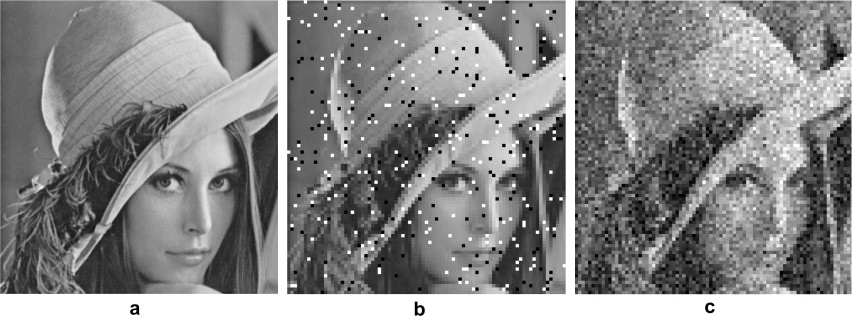
\includegraphics[width=0.8\textwidth]{./imgs/figura0.png}
	\caption{}
	\fonte{\cite{}}
\end{figure}

\begin{figure}[!htb]
	\centering
	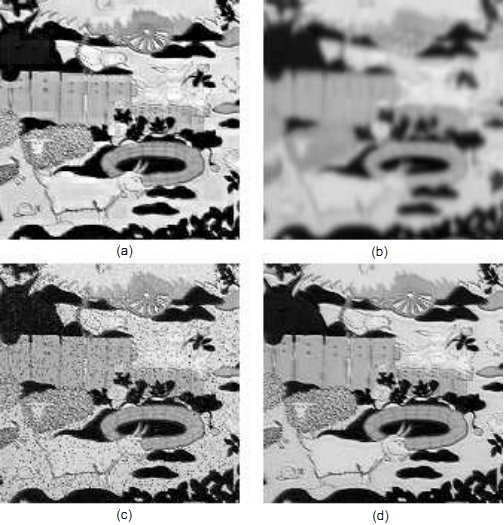
\includegraphics[width=0.8\textwidth]{./imgs/figura1.png}
	\caption{Principais artefatos em vídeos digitais: (a) blocagem; (b) embaraçamento; (c) ruído e (d) efeito vibrante.}
	\fonte{\cite{farias2007}}
\end{figure}

\section{Tecnologias}
